%%%%%%%%%%%%%%
%% Run LaTeX on this file several times to get Table of Contents,
%% cross-references, and citations.

%% If you have font problems, you may edit the w-bookps.sty file
%% to customize the font names to match those on your system.

%% w-bksamp.tex. Current Version: Feb 16, 2012
%%%%%%%%%%%%%%%%%%%%%%%%%%%%%%%%%%%%%%%%%%%%%%%%%%%%%%%%%%%%%%%%
%
%  Sample file for
%  Wiley Book Style, Design No.: SD 001B, 7x10
%  Wiley Book Style, Design No.: SD 004B, 6x9
%
%
%  Prepared by Amy Hendrickson, TeXnology Inc.
%  http://www.texnology.com
%%%%%%%%%%%%%%%%%%%%%%%%%%%%%%%%%%%%%%%%%%%%%%%%%%%%%%%%%%%%%%%%

%%%%%%%%%%%%%
% 7x10
%\documentclass{wileySev}

% 6x9

\documentclass{wileysix}
\UseRawInputEncoding
\usepackage{graphicx}
\usepackage{listings}

\usepackage{float}

\usepackage{color}

%\usepackage[b5paper]{geometry}
 
\definecolor{codegreen}{rgb}{0,0.6,0}
\definecolor{codegray}{rgb}{0.5,0.5,0.5}
\definecolor{codepurple}{rgb}{0.58,0,0.82}
\definecolor{backcolour}{rgb}{0.95,0.95,0.92}
 
\lstdefinestyle{mystyle}{
    backgroundcolor=\color{backcolour},   
    commentstyle=\color{codegreen},
    keywordstyle=\color{magenta},
    numberstyle=\tiny\color{codegray},
    stringstyle=\color{codepurple},
    basicstyle=\footnotesize,
    breakatwhitespace=false,         
    breaklines=true,                 
    captionpos=b,                    
    keepspaces=true,                 
    numbers=left,                    
    numbersep=5pt,                  
    showspaces=false,                
    showstringspaces=false,
    showtabs=false,                  
    tabsize=2,
    language=sh
}
 
\lstset{style=mystyle}

%%%%%%%
%% for times math: However, this package disables bold math (!)
%% \mathbf{x} will still work, but you will not have bold math
%% in section heads or chapter titles. If you don't use math
%% in those environments, mathptmx might be a good choice.

% \usepackage{mathptmx}

% For PostScript text
\usepackage{w-bookps}

%%%%%%%%%%%%%%%%%%%%%%%%%%%%%%%%%%%%%%%%%%%%%%%%%%%%%%%%%%%%%%%%
%% Other packages you might want to use:

% for chapter bibliography made with BibTeX
% \usepackage{chapterbib}

% for multiple indices
% \usepackage{multind}

% for answers to problems
% \usepackage{answers}

%%%%%%%%%%%%%%%%%%%%%%%%%%%%%%
%% Change options here if you want:
%%
%% How many levels of section head would you like numbered?
%% 0= no section numbers, 1= section, 2= subsection, 3= subsubsection
%%==>>
\setcounter{secnumdepth}{3}

%% How many levels of section head would you like to appear in the
%% Table of Contents?
%% 0= chapter titles, 1= section titles, 2= subsection titles, 
%% 3= subsubsection titles.
%%==>>
\setcounter{tocdepth}{2}

%% Cropmarks? good for final page makeup
%% \docropmarks

%%%%%%%%%%%%%%%%%%%%%%%%%%%%%%
%
% DRAFT
%
% Uncomment to get double spacing between lines, current date and time
% printed at bottom of page.
% \draft
% (If you want to keep tables from becoming double spaced also uncomment
% this):
% \renewcommand{\arraystretch}{0.6}
%%%%%%%%%%%%%%%%%%%%%%%%%%%%%%

%%%%%%% Demo of section head containing sample macro:
%% To get a macro to expand correctly in a section head, with upper and
%% lower case math, put the definition and set the box 
%% before \begin{document}, so that when it appears in the 
%% table of contents it will also work:

\newcommand{\VT}[1]{\ensuremath{{V_{T#1}}}}

%% use a box to expand the macro before we put it into the section head:

\newbox\sectsavebox
\setbox\sectsavebox=\hbox{\boldmath\VT{xyz}}

%%%%%%%%%%%%%%%%% End Demo


\begin{document}


\booktitle{Dasar - Dasar Android}
\subtitle{}

\authors{Faris Muhammad Ihsan\\
Syabriena Putri Veriane\\
\affil{Politeknik Pos Indonesia}
%Floyd J. Fowler, Jr.\\
%\affil{University of New Mexico}
}

%\offprintinfo{Cerdas Menguasai Git, First Edition}{Rolly M. Awangga}

%% Can use \\ if title, and edition are too wide, ie,
%% \offprintinfo{Survey Methodology,\\ Second Edition}{Robert M. Groves}

%%%%%%%%%%%%%%%%%%%%%%%%%%%%%%
%% 
\halftitlepage

\titlepage


\begin{copyrightpage}{2019}
%Survey Methodology / Robert M. Groves . . . [et al.].
%\       p. cm.---(Wiley series in survey methodology)
%\    ``Wiley-Interscience."
%\    Includes bibliographical references and index.
%\    ISBN 0-471-48348-6 (pbk.)
%\    1. Surveys---Methodology.  2. Social 
%\  sciences---Research---Statistical methods.  I. Groves, Robert M.  II. %
%Series.\\
%
%HA31.2.S873 2007
%001.4'33---dc22                                             2004044064
\end{copyrightpage}

%%%%%%%%%%%%%%%%%%%%%%%%%%%%%%%%%%%%%%%%%%%%%%%%%%%%%%%%%%%%%%%%%
%% \dedication{`Jika Kamu tidak dapat menahan lelahnya belajar, 
%% aka kamu harus sanggup menahan perihnya Kebodohan.'
%% ~Imam Syafi'i~}
%%%%%%%%%%%%%%%%%%%%%%%%%%%%%%%%%%%%%%%%%%%%%%%%%%%%%%%%%%%%%%%%%%

%\begin{contributors}
%\name{Rolly Maulana Awangga,} Informatics Research Center., Politeknik Pos Indonesia, Bandung,
Indonesia



%\end{contributors}

\contentsinbrief
\tableofcontents
\listoffigures
\listoftables
\lstlistoflistings


\begin{foreword}
Sepatah kata dari Kaprodi, Kabag Kemahasiswaan dan Mahasiswa
\end{foreword}

\begin{preface}
Buku ini diciptakan bagi yang awam dengan git sekalipun.

\prefaceauthor{R. M. Awangga}
\where{Bandung, Jawa Barat\\
Februari, 2019}
\end{preface}


\begin{acknowledgments}
Terima kasih atas semua masukan dari para mahasiswa agar bisa membuat buku ini 
lebih baik dan lebih mudah dimengerti.

Terima kasih ini juga ditujukan khusus untuk team IRC yang 
telah fokus untuk belajar dan memahami bagaimana buku ini mendampingi proses 
Intership.
\authorinitials{R. M. A.}
\end{acknowledgments}

\begin{acronyms}
\acro{ACGIH}{American Conference of Governmental Industrial Hygienists}
\acro{AEC}{Atomic Energy Commission}
\acro{OSHA}{Occupational Health and Safety Commission}
\acro{SAMA}{Scientific Apparatus Makers Association}
\end{acronyms}

\begin{glossary}
\term{git}Merupakan manajemen sumber kode yang dibuat oleh linus torvald.

\term{bash}Merupakan bahasa sistem operasi berbasiskan *NIX.

\term{linux}Sistem operasi berbasis sumber kode terbuka yang dibuat oleh Linus Torvald
\end{glossary}

\begin{symbols}
\term{A}Amplitude

\term{\hbox{\&}}Propositional logic symbol 

\term{a}Filter Coefficient

\bigskip

\term{\mathcal{B}}Number of Beats
\end{symbols}

\begin{introduction}

%% optional, but if you want to list author:

\introauthor{Rolly Maulana Awangga, S.T., M.T.}
{Informatics Research Center\\
Bandung, Jawa Barat, Indonesia}

Pada era disruptif  \index{disruptif}\index{disruptif!modern} 
saat ini. git merupakan sebuah kebutuhan dalam sebuah organisasi pengembangan perangkat lunak.
Buku ini diharapkan bisa menjadi penghantar para programmer, analis, IT Operation dan Project Manajer.
Dalam melakukan implementasi git pada diri dan organisasinya.

Rumusnya cuman sebagai contoh aja biar keren\cite{awangga2018sampeu} \cite{maulani2018analysis}.

\begin{equation}
ABC {\cal DEF} \alpha\beta\Gamma\Delta\sum^{abc}_{def}
\end{equation}

\end{introduction}

%%%%%%%%%%%%%%%%%%Isi Buku_

\chapter{Android}
\chapter{\textit{Android}}

\section{Sejarah \textit{Android}}

\begin{figure}[]
    \centering
    
\includegraphics[scale=0.2]{pictures/logo_android.jpg}
    \caption{Logo}
\end{figure}

Android merupakan sistem operasi berbasis linux yang dirancang untuk perangkat bergerak atau layar sentuh seperti \textit{smartphone} dan \textit{tablet}. Android adalah sistem operasi dengan sumber terbuka, dan Google merilis kodenya di bawah Lisensi Apache. Lisensi Apache adalah sebuah lisensi perangkat lunak-bebas yang ditulis oleh Apache Software Foundation (ASF). Android didirikan di Palo Alto, California pada bulan Oktober tahun 1980 oleh Andy Rubin, Rich Muner, Nick Sears, dan Chris White. Awalnya android dikembangkan oleh perusahaan yang bernama \textit{Android, Inc} yang mendapat dukungan finansial dari \textit{Google}, yang kemudian dibeli oleh \textit{Google} pada tahun 2005. Android awalnya tidak dibuat untuk ponsel, melainkan android dibuat untuk kamera digital. Karena peluang pada perangkat mobile lebih besar untuk berkembangjadi Android diplot untuk menyaingi Symbian dan Windows Mobile.

Android secara resmi dirilis pada tahun 2007 bersamaan dengan didirikannya \textit{Open Handset Alliance}. \textit{Open Handset Alliance} adalah pengembangan standar terbuka bagi perangkat selular. Pada tahun 2008 HP pertama yang menggunakan sistem operasi android akhirnya dirilis, yaitu HTC Dream. Dua tahun berselang, Google melepaskan ponsel pintar seri Nexus One yang proses pembuatannya dibantu oleh HTC. Kemudian muncul berbagai brand dari OEM yang berbeda mulai dari Samsung, LG, Asus, Lenovo, HTC, dan lain sebagainya. Selain pada \textit{smartphone}, Google juga mengembangkan Android TV untuk televisi, Android Auto untuk mobil, dan Android Wear untuk jam tangan, yang masing-masing memiliki interface yang berbeda. Kode dengan sumber terbuka dan lisensi perizinan pada Android memungkinkan perangkat lunak untuk dimodifikasi secara bebas dan didistribusikan oleh para pembuat perangkat, operator nirkabel, dan pengembang aplikasi. Selain itu, Android memiliki sejumlah besar komunitas pengembang aplikasi (apps) yang memperluas fungsionalitas perangkat, umumnya ditulis dalam versi kustomisasi bahasa pemrograman Java. Pada bulan Oktober 2013, ada lebih dari satu juta aplikasi yang tersedia untuk Android, dan sekitar 50 miliar aplikasi telah diunduh dari Google Play, toko aplikasi utama Android.\\
\\
Sejak tahun 2008, Android secara bertahap telah melakukan sejumlah pembaruan untuk meningkatkan kinerja sistem operasi, menambahkan fitur baru, dan memperbaiki bug yang terdapat pada versi sebelumnya. Setiap versi utama yang dirilis dinamakan secara alfabetis berdasarkan nama-nama makanan pencuci mulut atau camilan bergula; misalnya, versi 1.5 bernama Cupcake, yang kemudian diikuti oleh versi 1.6 Donut. Versi terbaru adalah 9.0 Pie, yang dirilis pada 7 maret 2018

\section{Versi Pada Android}
Sejak awal dipublikasikan, Android telah mempunyai banyak versi. Berbagai versi android dengan fitur-fitur keunggulannya masing-masing. Hal ini tentu disamping dengan pesaingnya yang sudah lama eksis, seperti Apple iOS, Windows, Blackberry (BB), Symbian dan sebagainya. Uniknya, setiap versi Android yang baru diluncurkan pasti selalu disertai dengan nama lucu yang sama sekali tidak ada hubungannya dengan karakter robot hijau (Android) tersebut.

\begin{enumerate}

\item Android 1.0 \textbf{Apple Pie}

Android versi pertama yaitu Apple Pie, yang dirilis pada 23 September 2008 dan hanya dilengkapi berbagai fitur seperti Play Store, kamera, Web Browser, Sinkronisasi antara G-mail, Contacts dan Google Agenda. Selain itu, diawal peluncurannya, Android juga sudah dilengkapi aplikasi Google Maps dan dukungan streaming Youtube. Google dan OHA merilis setidaknya ada 2 versi sebelum Android beta dirilis pada November 2007. Versi Alpha memiliki codename yaitu : Astro Boy, Bender dan R2-D2.\\
\\

\begin{figure}[]
    \centering
    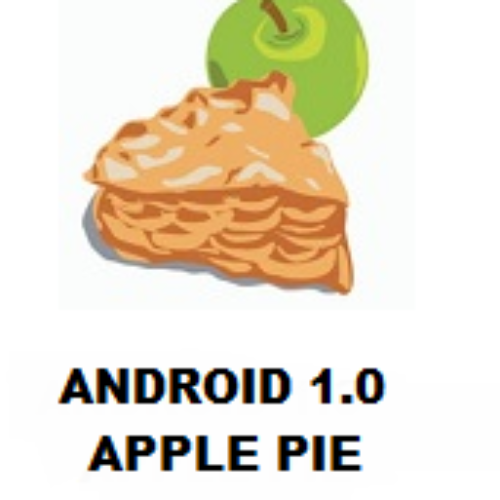
\includegraphics[scale = 0.3]{pictures/asd.jpg}
    \caption{Android Apple Pie}
    \label{}
\end{figure}
KELEBIHAN\\
\begin{enumerate}

\item Android Market, untuk mengunduh dan memperbarui aplikasi melalui toko aplikasi resmi Android.
\item Penjelajah web, untuk menampilkan, memperbesar dan melihat dalam layar penuh halaman web HTML dan XHTML.
\item Dukungan kamera, versi ini tidak memiliki pilihan untuk mengubah resolusi kamera, kejernihan, kualitas foto, dan sebagainya.
\item Memungkinkan pengelompokan sejumlah ikon aplikasi ke dalam satu folder di layar depan (homescreen).
\item Akses ke server surel web, mendukung POP3, IMAP4, dan SMTP
\item Sinkronisasi Gmail dengan aplikasi Gmail.
\item Sinkronisasi Google Contacts dengan aplikasi People
\item Sinkronisasi Google Calendar dengan aplikasi Calendar
\item Google Maps, dengan Latitude dan Street View untuk melihat peta dan citra satelit, serta menemukan lokasi bisnis dan petunjuk arah mengemudi dengan menggunakan GPS.
\item Google Sync, memungkinkan pengelolaan sinkronisasi pada aplikasi Gmail, People, dan Calendar.
\item Google Search, memungkinkan pengguna untuk mencari sesuatu di Internet.
\item Google Talk, aplikasi pesan instan.
\item Pesan instan, pesan teks (SMS), dan MMS.
\item Pemutar media, untuk mengelola, mengimpor, dan memutar berkas media, namun versi ini tidak menyediakan dukungan video dan Bluetooth stereo.
\item Notifikasi muncul pada status bar, dengan pilihan untuk mengatur nada dering, LED, atau nada getar.
\item Voice Dialer, memungkinkan pengguna untuk memanggil kontak tanpa harus mengetik nama atau nomor telepon.
\item Wallpaper, memungkinkan pengguna untuk mengatur gambar latar belakang di layar depan.
\item Pemutar video YouTube.
\item Aplikasi lainnya seperti: Jam Alarm, Kalkulator, Panggilan, Home screen (Launcher), Galeri, dan Pengaturan.
\item Dukungan Wi-Fi dan Bluetooth.
\end{enumerate}

KEKURANGAN\\
\begin{enumerate}
    \item versi ini android belum memiliki nama sehinggan masih belum mudah diingat masyarakat.
\end{enumerate}


\item Android 1.1 \textbf{Banana Bread}\\
Sistem Operasi android yang rilis selanjutnya yaitu Banana Bread, rilis pada bulan Februari 2009. Dan fiturnya yaitu tidak jauh berbeda dengan versi sebelumnya. HTC merupakan salah satu smartphone Android pertama yang menggunakan versi ini. Android 1.1 juga dikenal dengan “Petit Four“, meskipun nama ini tidak digunakan secara resmi. Versi ini memperbaiki beberapa bug, mengubah API Android, dan menambahkan beberapa fitur:
\begin{enumerate}
    \item Rincian dan tinjauan tersedia saat pengguna mencari lokasi bisnis pada Peta.
    \item Kemampuan untuk menampilkan/meenyembunyikan tombol panggilan.
    \item Kemampuan untuk menyimpan lampiran pada pesan.
    \item Menambah dukungan marquee pada tata ruang sistem.
\end{enumerate}


\item Android 1.5 \textbf{Cupcake}\\
Dirilis pada awal bulan April 2009 dan juga tidak berbeda dengan versi Android sebelumnya. Hanya saja terdapat fitur tambahan seperti sudah Support Bluetooth A2DP, AVRCP, Soft-keyboard dengan prediksi text dan record atau watch videos. ersi ini adalah rilis pertama yang secara resmi menggunakan nama kode berdasarkan nama-nama makanan pencuci mulut (“Cupcake”), nama yang kemudian digunakan untuk semua versi rilis selanjutnya. Pembaruan pada versi ini termasuk beberapa fitur baru dan perubahan UI:
\begin{enumerate}
    \item Dukungan papan ketik virtual pihak ketiga dengan prediksi teks dan kamus pengguna
    \item Dukungan Widget – tampilan aplikasi miniatur yang tertanam dalam aplikasi lain dan menerima pembaruan secara periodik
    \item Kemampuan merekam dan memutar video berformat MPEG-4 dan 3GP
    \item Kemampuan memasangkan (pairing) dan dukungan stereo bagi Bluetooth (A2DP dan AVRCP)
    \item Fitur salin dan tempel pada penjelajah web
    \item Foto pengguna ditampilkan pada kontak favorit
    \item Tanggal/waktu ditampilkan pada log panggilan, dan akses satu sentuhan ke nomor kontak dari log panggilan
    \item Transisi layar animasi
    \item Opsi memutar-otomatis
    \item Animasi boot baru
    \item Kemampuan untuk mengunggah video ke YouTube
    \item Kemampuan untuk mengunggah foto ke Picasa
\end{enumerate}


\item Android 1.6 \textbf{Donut}\\
\begin{figure}[]
    \centering
    
\includegraphics[scale=0.5]{pictures/android_donut.jpg}
    \caption{Logo Android Donut}
    \label{}
\end{figure}
Android Donut dirilis pada 15 September 2009, dan terdapat fitur tambahan seperti Gesture Framework hingga Turn-by-turn navigation. Kemudian, Android ini juga terlihat lebih sempurna pada saat itu. Dengan minimnya bug, ditambah lebih lengkapnya berbagai fitur yang disediakan oleh Google. Fitur-fitur barunya adalah sebagai berikut:
\begin{enumerate}
    \item Entri pencarian teks dan suara diperluas, termasuk menyertakan riwayat bookmark, kontak, dan web
    \item Kemampuan bagi para pengembang untuk menyertakan konten mereka pada hasil pencarian
    \item Mesin sintesis pengucapan multibahasa yang memungkinkan aplikasi Android tertentu mampu mengucapkan teks
    \item Pencarian yang lebih mudah dan kemampuan untuk melihat cuplikan aplikasi di Android Market
    \item Galeri, kamera, dan perekam video yang lebih terintegrasi, dengan akses kamera yang lebih cepat
    \item Kemampuan memilih banyak foto untuk dihapus
    Pembaruan dukungan teknologi bagi CDMA/EVDO, 802.1x, VPN, dan mesin pengucap teks
    \item Dukungan bagi resolusi layar WVGA
    \item Peningkatan kecepatan dalam pencarian dan aplikasi kamera
    \item Perluasan kerangka kerja Gestur dan penambahan perkakas pengembangan GestureBuilder.
\end{enumerate}

KEKURANGAN\\
\begin{enumerate}
    \item Tidak semua aplikasi (.apk) bisa di install di sini.
    \item Music playernya belum ada equalizernya.
    \item Android market yang tidak integrated
    \item Keypad nya lemot dan touch responsiveness nya kurang sip daripada versi sesudahnya
\end{enumerate}


\item Android 2.0 \textbf{Eclair} (API level 5)\\
\begin{figure}[]
    \centering
    
\includegraphics[scale=0.3]{pictures/android-eclair.jpg}
    \caption{Logo Android Eclair}
    \label{}
\end{figure}
Android versi 2.0 ini bernama Eclair dan dirilis pada 26 Oktober 2009 silam. Selain terdapat bluetooth, versi ini juga mendapatkan fitur tambahan seperti multi-touch, Live Wallpaper dan juga flash kamera. Kemudian, beberapa fitur yang dapat anda nikmati dalam versi eclair adalah HTML, Digital zoom, Support Microsoft Exchange, dan Updated UI. Perubahan pada versi ini meliputi:
\begin{enumerate}
    \item Sinkronisasi akun diperluas, yang memungkinkan pengguna menambahkan beberapa akun untuk sinkronisasi surel dan kontak
    \item Dukungan surel Microsoft Exchange, dengan kemampuan menjelajah surel dari beberapa akun dalam satu halaman
    \item Dukungan Bluetooth 2.1
    \item Kemampuan untuk memilih foto kontak dan opsi untuk memanggil, mengirim SMS atau surel kepada kontak yang bersangkutan
    \item Kemampuan untuk mencari semua SMS dan MMS tersimpan, pesan terlama akan dihapus jika batas yang ditentukan sudah tercapai.
    \item Menambahkan sejumlah fitur pada kamera, termasuk dukungan kilat (flash), perbesaran digital, mode skin, kejernihan, efek warna, dan fokus makro.
    \item Peningkatan kecepatan mengetik pada papan ketik virtual, dengan dukungan kamus yang mempelajari penggunaan kata-kata, termasuk nama kontak sebagai saran
    \item UI penjelajah web yang baru, dengan fitur bookmark thumbnail, double-tap zoom, dan dukungan bagi HTML5
    \item Penyempurnaan tampilan agenda kalender; menampilkan status menghadiri untuk setiap undangan, dan kemampuan untuk mengundang tamu baru ke acara tertentu
    \item Mengoptimalkan kecepatan perangkat lunak dan perubahan UI
    \item Dukungan bagi lebih banyak resolusi dan ukuran layar, dengan rasio kecerahan yang lebih baik
    \item Peningkatan Google Maps 3.1.2
    \item MotionEvent ditingkatkan untuk melacak aktivitas multisentuh
    \item Penambahan live wallpaper, yang menampilkan animasi pada latar belakang layar depan
\end{enumerate}

\item Android 2.0.1 \textbf{Eclair} (API level 6)\\
Android versi 2.0 ini bernama Eclair dan dirilis pada 3 Desember 2009. Fitur pada versi ini yaitu :
\begin{enumerate}
    \item Perubahan API minor
    \item Perbaikan bug
    \item perubahan kerangka kerja.
\end{enumerate}

\item Android 2.1 \textbf{Eclair} (API level 7)\\
Android versi 2.0 ini bernama Eclair dan dirilis pada 12 Januari 2010. Fitur pada versi ini yaitu :
\begin{enumerate}
    \item Perubahan kecil pada API 
    \item Perbaikan bug
\end{enumerate}

\item Android 2.2 9 \textbf{Froyo}\\
Pada bulan Mei 2010 lalu, Perusahaan raksasa Google telah merilis Android versi terbaru Yakni adalah Android 2.2 9 (Froyo). Versi ini adalah salah satu sistem operasi Android yang juga telah disempurnakan, tujuannya tentu untuk meningkatkan kecepatan kinerja suatu sistem Android. Dan berikut ini adalah beberapa fitur dan perbaikan yang disediakan oleh Android Froyo :
\begin{enumerate}
    \item Peningkatan Speed
    \item Implementasi JIT
    \item Integrasi mesin JavaScript V8 Chrome pada aplikasi penjelajah web
    \item Dukungan bagi layanan Android Cloud to Device Messaging (C2DM)
    \item Peningkatan dukungan Microsoft Exchange, termasuk kebijakan keamanan, pencarian otomatis, GAL, sinkronisasi kalender, dan pembersihan jarak jauh
    \item Peningkatan peluncur aplikasi dengan jalan pintas ke Telepon dan aplikasi penjelajah web
    \item USB Tethering
    \item Opsi untuk mematikan akses data pada jaringan seluler
    \item Pembaruan aplikasi Market dengan menambahkan fitur pembaruan otomatis
    \item Kontak dan panggilan suara bisa dibagikan melalui Bluetooth
    \item Dukungan bagi Bluetooth-enabled car dan desk docks
    \item Dukungan bagi sejumlah kata sandi alfanumerik
    \item Aplikasi instalasi untuk perluasan memori atau storange
    \item Support file upload pada aplikasi browser
    \item Animated GIFs
    \item Dukungan Adobe Flash
    \item Dukungan tampilan PPI (hingga 320 ppi), misalnya layar 4″ 720p
    \item Gestur pembesaran pada Galeri
\end{enumerate}

\item Android 2.3 \textbf{Gingerbread}\\
Pada bulan Desember 2010 lalu, Google merilis kembali Android versi terbarunya yaitu Gingerbread. Yang secara fitur sudah jelas sangat sempurna. Ditambah lagi, Android 2.3 ini juga telah diadopsi oleh salah satu perusahaan Smartphone paling populer, yaitu Samsung dengan menanamkan sistem operasi ini dalam smartphone seri Nexus-nya. Fitur yang disediakan :
\begin{enumerate} 
    \item Memperbarui desain antarmuka pengguna dengan meningkatkan kecepatan dan kesederhanaan
    \item Dukungan bagi resolusi dan ukuran layar ekstra-besar (WXGA dan yang lebih tinggi)
    \item Dukungan bagi telepon internet SIP VoIP
    \item Masukan teks yang lebih cepat dan lebih intuitif pada papan ketik virtual, dengan meningkatkan akurasi, saran teks yang lebih baik, dan modus input suara
    \item Peningkatan fungsi salin/tempel, memungkinkan pengguna untuk memilih kata dengan menekan dan menahan layar
    \item Dukungan bagi Near Field Communication (NFC), memungkinkan pengguna untuk membaca tag NFC yang tertanam dalam poster, stiker, atau iklan
    \item Efek audio baru seperti reverb, equalizer, virtualisasi penyuara kuping, dan bass boost
    \item Download Manager baru, memudahkan pengguna untuk mengakses berkas yang diunduh dari penjelajah web, surel, ataupun dari aplikasi lainnya
    \item Dukungan multi kamera pada perangkat, termasuk kamera depan, jika tersedia
    \item Dukungan bagi pemutar video WebM/VP8, dan audio AAC
    \item Peningkatan manajemen daya dengan peran lebih aktif dalam mengelola aplikasi yang beroperasi terlalu lama
    \item Peningkatan dukungan bagi pengembangan kode asli
    \item Peralihan dari YAFFS ke ext4 pada perangkat yang lebih baru
    \item Peningkatan kualitas audio, grafis, dan masukan bagi pengembang permainan
    \item Dukungan sensor yang lebih banyak (seperti giroskop dan barometer)
\end{enumerate}

\item Android 3.0 - 3.2 6 \textbf{Honeycomb}\\
\item \begin{figure}[]
    \centering
    
\includegraphics[scale=0.1]{pictures/android-honeycomb.png}
    \caption{}
    \label{}
\end{figure}
Honeycomb adalah salah satu sistem operasi Android versi terbaru yang dirilis pada bulan Februari 2011 silam. Namun, versi ini lebih ditujukkan untuk perangkat Tablet yang mana pada tahun itu sangat laris atau laku dipasaran. Beberapa fitur dan perbaikan pada Android Honeycomb, yaitu :
\begin{enumerate}
    \item Support Multi core
    \item Support Tablet lebih baik
    \item Updated 3D UI
    \item Layar Utama (homescreens) yang dapat diatur
    \item Melihat aplikasi yang barusan dibuka
    \item Menyempurnakan layout keyboard
    \item Transport protocol untuk Media atau Picture video chat Google Talk
    \item Google eBooks
    \item “Private browsing”
    \item System-wide Clipboard
    \item HTTP Live streaming
\end{enumerate}
Update 3.1:
\begin{enumerate}
    \item Peningkatan UI
    \item Open Accessory API
    \item USB host API
    \item Support mouse, joysticks dan gamepad
    \item Widget Home screen yang bisa di atur size atau ukurannya
    \item Notificasi MTP
    \item RTP API untuk audio
\end{enumerate}
Update 3.2:
\begin{enumerate}
    \item Optimise pada berbagai tablets
    \item Mode kompatibilitas display (zoom for fixed sized apps)
    \item Sinkronisasi Media dari SD card
\end{enumerate}
Update 3.2.1:
\begin{enumerate}
    \item Update Android Market merupakan automatic updates yang lebih mudah
    \item Update Google Books
    \item Peningkatan kinerja Wi-Fi
    \item Perbaikan prediksi tulisan tangan dengan huruf Chinese
\end{enumerate}
Update 3.2.2:
\begin{enumerate}
    \item Perbaikan kecil
\end{enumerate}
Update 3.2.4:
\begin{enumerate}
    \item Update tambahan ‘Pay as you go’ bagi tablet
\end{enumerate}
Update 3.2.6
\begin{enumerate}
    \item Perbaikan kecil 
\end{enumerate}

\item Android 4.0 \textbf{Ice Cream Sandwich}\\
Puncak kesempurnaan Android yakni ketika pada versi ini, dimana Ice Cream Sandwich dirilis pada bulan Oktober 2011 silam. Dan operasi sistem ini mulai bekerja dengan baik di semua jenis smartphone apapun. Selain bertambahnya berbagai fitur yang menarik, Ice Cream Sandwich juga merupakan versi yang paling banyak disukai pada saat itu. Bahkan, Android Ice Cream Sandwich juga sudah dilengkapi dengan fitur ekstra multitasking serta notifikasi yang lebih banyak. Pembaruan pada versi ini antara lain:
\begin{enumerate}
    \item Tombol lunak tablet Android 3.x tersedia bagi penggunaan di telepon pintar
    \item Pemisahan widget di tab baru, terletak pada layar yang bersebelahan dengan aplikasi
    \item Pembuatan folder yang lebih mudah, dengan gaya drag-and-drop
    \item Launcher yang bisa dikustomisasi
    \item Peningkatan fitur pesan suara visual, dengan kemampuan untuk mempercepat atau memperlambat kecepatan pesan suara
    \item Fungsi ‘cubit untuk memperbesar’ pada kalender
    \item Pengintegrasian fungsi cuplikan layar (screenshot) dengan menekan dan menahan tombol daya dan volume-turun secara bersamaan
    \item Perbaikan kesalahan koreksi pada papan ketik
    \item Kemampuan untuk mengakses aplikasi secara langsung dari layar kunci (lock screen)
    \item Perbaikan fungsi salin dan tempel
    \item Integrasi suara yang lebih baik dan berkesinambungan
    \item Mode buka kunci identifikasi wajah, fitur yang memungkinkan pengguna untuk membuka perangkat menggunakan perangkat lunak pengenal wajah
    \item Penambahan penjelajah web bawaan Chrome, mampu membuka halaman hingga 16 tab
    \item Sinkronisasi otomatis pada penjelajah web dengan bookmark Chrome pengguna
    \item Penambahan jenis huruf baru, Roboto
    \item Penggunaan data bisa dibatasi, pengguna akan diperingatkan jika penggunaan data sudah mendekati batas tertentu, dan menonaktifkan data yang digunakan ketika batas tersebut terlampaui
    \item Kemampuan untuk mematikan aplikasi yang menggunakan data di latar belakang
    \item Peningkatan fungsi aplikasi kamera dengan fitur-fitur seperti zero shutter lag, time lapse settings, mode panorama, dan kemampuan untuk memperbesar saat merekam video
    \item Penambahan aplikasi pengedit foto bawaan
    \item Tata letak galeri yang baru, bisa dikelola berdasarkan lokasi dan orang
    \item Pemutakhiran aplikasi “People” dengan integrasi pada jejaring sosial
    \item Android Beam, fitur komunikasi area dekat yang memungkinkan dilakukannya pertukaran jarak pendek bookmark web, info kontak, arah, video YouTube, dan data lainnya
    \item Dukungan format gambar WebP
    \item Merekam video 1080p bagi perangkat Android tertentu
    \item Modul kernel Android VPN Framework (AVF) dan TUN (bukan TAP). Sebelum versi 4.0, perangkat lunak VPN membutuhkan rooting.
\end{enumerate}

\item Android 4.1.2 \textbf{Jelly Bean}\\
Jelly Bean dirilis pada 9 Juli 2012 lewat konferensi I/O Google. Versi ini adalah salah satu versi Android yang kerap mendapatkan update fitur-fitur yang bermanfaat dan menarik, beberapa contohnya semacam memperbaiki rotasi layar, seperti Support resolusi video 4K, Support penulisan huruf Hebrew dan Arabic dari kanan ke kiri, peningkatan kinerja, dan sistem keamanan serta masih banyak lainnya. Fitur yang terdapat pada versi ini adalah : 
\begin{enumerate}
    \item Antarmuka pengguna yang lebih halus:
    \item Waktu vsync pada animasi UI dikelola oleh kerangka kerja Android, termasuk reaksi aplikasi, efek sentuh, komposisi layar, dan penyegaran tampilan
    \item Triple buffering pada grafis
    \item Peningkatan aksesbilitas
    \item Teks dua bahasa dan dukungan bahasa lainnya
    \item Papan ketik yang bisa dimodifikasi oleh pengguna
    \item Perluasan notifikasi
    \item Kemampuan untuk mematikan notifikasi pada aplikasi tertentu
    \item Shortcut dan widget secara otomatis bisa disusun ulang atau diatur ukurannya
    \item Transfer data Bluetooth bagi Android Beam
    \item Diktasi suara luring
    \item Tablet dengan layar kecil bisa menyesuaikan tata letak antarmuka dan layar depan seperti pada telepon pintar
    \item Peningkatan pencarian suara
    \item Peningkatan aplikasi kamera
    \item Google Wallet (pada Nexus 7)
    \item Foto kontak Google+ resolusi tinggi
    \item Aplikasi pencarian Google Now
    \item Audio multi-saluran
    \item Audio USB (bagi suara eksternal DACs)
    \item Audio chaining
    \item Penjelajah web bawaan Android diganti dengan Google Chrome pada perangkat Android pra-instal
    \item Kemampuan untuk menambahkan widget aplikasi tanpa akses root
\end{enumerate}

\item Android 4.4 \textbf{Kitkat}\\
Android versi inilah yang saat ini banyak dipakai oleh mayoritas masyarakat Indonesia. Kitkat dirilis pada tahun 2013 lalu. pada versi ini, Android banyak mendapatkan pembaharuan/update fitur. Seperti, terdapatnya fitur Screen recording, untuk merekam kegiatan yang terjadi pada layar smartphone, Peningkatan akses notifikasi, New Translucent system UI, System wide settings untuk closed captioning, dan Peningkatan kinerja serta lain sebagainya. Fitur yang terdapat pada versi ini adalah : 
\begin{enumerate}
    \item Pembaruan antarmuka dengan bar status dan navigasi transparan pada layar depan.
    \item Optimasi kinerja pada perangkat dengan spesifikasi yang lebih rendah
    \item Kerangka kerja pencetakan
    \item NFC Host Card Emulation sebagai emulator kartu pintar
    \item WebViews berbasis Chromium
    \item Perluasan fungsionalitas bagi layanan pendengar notifikasi
    \item API umum untuk mengembangkan dan mengelola klien pesan teks, kemampuan untuk menentukan aplikasi SMS standar.
    \item Kerangka kerja baru untuk transisi UI
    \item Kerangka kerja akses penyimpanan untuk mengambil konten dan dokumen dari sumber lain
    \item Sensor batching, Step Detector, dan Counter API
    \item Peningkatan tampilan mode layar penuh, tombol perangkat lunak dan status bar bisa diakses dari tepi dengan cara menggesek
    \item Penyeimbang audio, pemantauan audio, dan peningkatan suara audio
    \item Perekam aktivitas layar yang terintegrasi
    \item Inframerah
    \item Peningkatan aksesibilitas API
    \item Mesin virtual eksperimental baru, ART
    \item Dukungan Bluetooth Message Access Profile (MAP)
\end{enumerate}

\item Android 5.0 \textbf{Lollipop}\\
Dirilis pada tahun 2014, Android Lollipop lebih banyak menawarkan fitur tambahan untuk menyempurnakan berbagai fitur yang sudah ada. Dan Nexus 6 merupakan salah satu ponsel yang pertama mencicipi Android Lollipon ini. Selain itu, Google juga lebih menyempurnakan pada kinerja dari Android Lollipop sendiri. Fitur yang terdapat pada versi ini adalah : 
\begin{enumerate}
    \item Desain antarmuka (tampilan) yang dinamakan “Material Design”.
    \item 64-bit ART compiler
    \item Project volta, yang berguna untuk meningkatkan daya hidup baterai 30 persen lebih tahan lama.
    \item ‘factory reset protection’. Fitur ini berguna ketika smartphone hilang, ia tidak bisa direset ulang tanpa memasukkan id google dan kata sandi (password).
\end{enumerate}

\item Android 6.0 \textbf{Marshmallow}\\
Android versi 6.0 dirilis pada tahun 2015 silam, yang banyak membawa pembaharuan. Salah satunya yaitu suda support USB Type-C. Selain itu, Android Marshmallow ini juga terdapat fasilitas autentikasi sidik jari dan daya baterai yang lebih baik. 

Android Marshmallow memperkenalkan model izin yang didesain ulang: sekarang ada hanya delapan kategori izin, dan aplikasi yang tidak lagi secara otomatis diberikan semua hak akses mereka ditentukan pada waktu instalasi. Sebuah sistem opt-in sekarang digunakan, di mana pengguna akan diminta untuk memberikan atau menolak izin individu (seperti kemampuan untuk mengakses kamera atau mikrofon) untuk aplikasi ketika mereka dibutuhkan. Aplikasi mengingat hibah izin mereka, dan mereka dapat disesuaikan oleh pengguna setiap saat. Model izin baru akan digunakan hanya oleh aplikasi yang dikompilasi untuk Marshmallow menggunakan kit pengembangan perangkat lunak (SDK) tersebut, sementara semua aplikasi lainnya akan terus menggunakan model izin sebelumnya.\\

Marshmallow juga memiliki skema manajemen daya baru bernama Doze yang mengurangi tingkat aktivitas aplikasi latar belakang saat perangkat menentukan bahwa itu tidak sedang aktif ditangani oleh pengguna, yang, menurut Google, menggandakan pemakaian baterai perangkat. Hal ini juga memperkenalkan pilihan untuk mengatur ulang semua pengaturan jaringan, tersedia untuk pertama kalinya pada Android, yang membersihkan pengaturan terkait jaringan untuk WI-FI, Bluetooth dan koneksi seluler.

Android Marshmallow memberikan dukungan asli untuk pengenalan sidik jari, memungkinkan penggunaan sidik jari untuk membuka perangkat dan otentikasi Play Store dan pembelian Android Pay; API standar juga tersedia untuk melaksanakan otentikasi berbasis sidik jari dalam aplikasi lain. Android Marshmallow mendukung USB Type-C, termasuk kemampuan untuk menginstruksikan perangkat untuk mengisi daya perangkat lain melalui USB. Marshmallow juga memperkenalkan “pranala yang diverifikasi” yang dapat dikonfigurasi untuk membuka langsung dalam aplikasi tertentu mereka tanpa petunjuk pengguna lanjut.

Versi API Android yang disediakan oleh Marshmallow adalah 23. Alat pengembang Android Marshmallow tersedia di Pengelola SDK di bawah tingkat API “MNC”.

\item Android 7.0 \textbf{Nougat}\\
Android Nougat versi 7.0 dirilis pada bulan Agustus 2016 yang lebih meningkatkan pada kinerja versi sebelumnya. Selain itu, Android Nougat juga menambah banyak fitur-fitur baru yang diantaranya seperti sudah dapat multitasking, meningkatkan fitur Doze yang dahulu telah dirilis di versi sebelumnya. Inilah beberapa fitur terbaru yang terdapat pada versi Nougat :
\begin{enumerate}
    \item Support Multi window
    \item Dapat langsung membalas pesan dari menu notifikasi atau jendela.
    \item Tampilan panel notifikasi serta quick settings yang baru.
    \item Mode Doze yang lebih baik, (Doze Mode 2.0)
    \item Menu di antara system settings.
\end{enumerate}

\item Android 8.0 \textbf{Oreo}
Android versi Oreo dirilis pada bulan Agustus 2017 lalu. Tentu saja Android Oreo merupakan versi final untuk sekarang ini. Beberapa fiturnya juga turut diluncurkan Google selaku pihak pengelola. Adapun fitur-fiturnya tersebut antara lain yaitu :
\begin{enumerate}
    \item Android O lebih berfokus pada kecepatan dan efisiensi
    \item Kecepatan Boot up 2X lebih cepat
    \item Mode Picture in picture lebih flexibel
    \item Aplikasi yang berjalan di latarbelakang atau background lebih diperketat untuk lebih menghemat battery
    \item Battery lebih tahan lama
    \item Emoji yang diperbaharui dan diperbanyak
\end{enumerate}
\end{enumerate}

\section{ Sejarah Android Studio}
\begin{figure}[]
    \centering
    
\includegraphics[scale=0.1]{pictures/android-studio.png}
    \caption{Android Studio}
    \label{}
\end{figure}
Pertama kali muncul Android Inc merupakan sebuah perusahaan software kecil yang didirikan pada bulan Oktober 2003 di Palo Alto, California, USA. Perusahaan ini dibangun oleh beberapa senior di beberpa perusahaan yang berbasis IT dan Communication, Andy Rubin, Rich Miner, Nick Sears dan Chris White. Rubin menyatakan bahwa, Android Inc Didirikan untuk mewujudkan mobile device yang lebih fleksibel terhadap lokasi dan preferensi pemilik. Sehingga, Android Inc ingin mewujudkan mobile device yang lebih mengerti pemiliknya selain karena OS nya yang open source. Berawal dari konsepan inilah Android Inc ternyata menarik minat Google untuk memilikinya. Maka, pada bulan Agustus 2005, Akhirnya Android Inc diakuisisi oleh Google Inc. dan seluruh sahamnya dibeli oleh Google.

Perusahaan milik Andy Rubin, Rich Miner, Nick Sears dan Chris White tetap di Android Inc yang dibeli Google, sehingga akhirnya mereka pun ikut  menjadi bagian dari raksasa Google dan sejarah Android. Disini mereka mulai menggunakan platform Linux untuk membuat sistem operasi bagi mobile phone.Dari sinilah akhirnya banyak pengembang sistem maupun software yang mengembangkan maupun merancang sistem Android menggunakan software – software yang support dengan Android, Contohnya ialah : Android Studio.

\chapter{Java}
\chapter{\textit{Java}}

\section{Sejarah \textit{Java}}

%\chapter{Judul Bagian Kedua}
%\section{Variabel}
Variabel adalah sebuah tempat untuk menampung value dimemori, dapat dimisalkan seperti sebuah ruangan atau wadah, variabel dibagi dua berdasarkan ruang lingkup yaitu variable lokal dan global, untuk menentukan variabel global atau lokal itu tergantung dari tempat dideklarasikannya variabel pada program yang sedang dibuat. Variabel global yaitu variabel yang dapat diakses di semua lingkup dalam program yang sedang dibuat, dalam kata lain variabel global ini dapat dikenali oleh semua fungsi dan prosedur, sementara variabel lokal yaitu variabel yang dapat diakses hanya di lingkup khusus, dalam kata lain variabel lokal ini hanya bisa diakses pada fungsi/prosedur dimana variabel itu dideklarasikan.
\par
Berikut merupakan standar-standar dalam penulisan variabel:
\begin{enumerate}
\item Nama variabel diawali dengan huruf atau garis bawah, contoh: nama, \_nama, namaKu, nama\_variabel.
\item Karakter selanjutnya dapat berupa huruf, garis bawah atau angka, contoh: \_\_nama, nama1, p1.
\item  Nama variabel tidak boleh diawali dengan angka
\item Karakter bersifat case-sensitive (huruf besar dan huruf kecil dibedakan), contoh: Nama dan NAMA keduanya memiliki arti yang berbeda dan merupakan variabel yang berbeda.
\item Nama variabel tidak boleh menggunakan kata kunci yang ada pada bahasa pemrograman python, contoh: if, else, while
\end{enumerate}

\section{Input dan Output}
Input \& output bertujuan agar pengguna dan program dapat berinteraksi,Perintah input() berguna untuk meminta inputan dari user, sehingga memungkinkan user untuk menginputkan data.\\
Perintah print() berguna untuk menampilkan output dari data yang diinputkan oleh user, sehingga data yang diinputkan user dapat ditampilkan ke layar.
\par
Contoh dari penggunaan input dan output adalah sebagai berikut:
\begin{lstlisting}[language=Python]
#Input yang ditujukan untuk user
nama=”informatics research center” 

#output yang didapatkan user
print(“Halo”, nama, ”selamat datang ”)
\end{lstlisting}

\section{Operasi Aritmatika}
Python memiliki operasi aritmatika, antara lainnya seperti :
\begin{enumerate}
\item penjumlahan (+)
\item pengurangan (-)
\item perkalian (*)
\item pembagian (/)
\item sisa bagi/modulus (\%)
\item pemangkatan (**)
\end{enumerate}
Penggunaan dari simbol simbol ini sama hal nya dengan fungsi aritmatika pada umumnya.

\section{Perulangan}
Dalam membuat sebuah program, terkadang kita memerlukan satu baris atau satu blok kode yang sama secara berulang, disini fungsi perulangan dipakai sehingga kita tidak perlu menulis baris atau blok kode yang sama secara terus menerus, dalam python perulangan dibagi menjadi 2, yaitu for dan while.

\subsection{For}
For merupakan perulangan yang akan mengulang kondisi true sampai batas yang telah ditentukan,  biasanya digunakan untuk perulangan yang mana parameter pengulangannya menggunakan list atau range. Berikut ini merupakan contoh penggunakan sintaks perulangan for.
\begin{lstlisting}[language=Python]
for i in range (0 ,10): 
		print( i )
\end{lstlisting}

\subsection{While}
While merupakan perulangan yang akan terjadi apabila kondisinya True, perulangan akan terus berjalan hingga diperoleh kondisi False.erikut ini merupakan contoh penggunakan sintaks perulangan while.
\begin{lstlisting}[language=Python]
#perulangan while
hitung = 0 
while (hitung < 9): 
  	print (’hitungan ke :’, hitung) 
  	hitung = hitung + 1
 
print ("Good bye!")
\end{lstlisting}

\section{Kondisi}
Pengambilan keputusan kadang diperlukan dalam sebuah program untuk menentukan tindakan apa yang akan dilakukan sesuai dengan kondisi yang terjadi, contoh kasus misalkan ada seorang anak bernama idam, seorang manusia yang membutuhkan makan, jika idam lapar maka idam akan makan. Maka dapat dijabarkan seperti dibawah ini :\\
\\
Kondisi, jika : \\
Idam lapar \\
Maka : \\
Idam akan makan\\
Namun terkadang kondisi juga diberikan tambahan opsi sebuah kondisi tambahan, misalkan jika idam makan maka idam kenyang, namun jika tidak maka idam akan kelaparan. Penjabarannya dapat dilihat sebagai berikut :\\
\\
Kondisi, jika :\\
 Idam makan \\
 Maka : \\
 Idam akan kenyang \\
 Jika tidak : \\
 Idam akan kelaparan\\
Contoh diatas dapat ditulis dalam sintax python dengan menggunakan kondisi, pengkondisiian dalam python dibagi menjadi 4, yaitu : IF, IF ELSE, ELIF, nested IF. Berikut merupakan pembahasannya.

\subsubsection{IF}
 IF  adalah suatu struktur yang memiliki suatu perlakuan jika terjadi suatu kondisi. Akan tetapi, tidak terjadi sesuatu yang lain atau terjadi apa-apa ketika berada di dalam luar kondisi tersebut. IF hanya menjalankan satu kondisi dan menampilkan satu output. Contoh: kondisi dimana variabel a lebih besar dari variabel b, maka tampilkan hasil bahwa a lebih besar dari b.
\begin{lstlisting}[language=Python]
#if statement 
a = 330 
b = 200 
if a > a: 
	print("a lebih besar dari b")
\end{lstlisting}

\subsubsection{IF ELSE}
IF ELSE digunakan apabila kondisi yang terjadi bernilai salah, maka lakukan else. Contoh: kondisi dimana variabel a lebih besar dari variabel b, maka jika b lebih besar dari a, tampiilkan hasil b lebih besar dari a, jika salah maka tampilkan a lebih besar dari pada b
\begin{lstlisting}[language=Python]
 #else 
a = 200 
b = 33 
if b > a: 
	print("b is greater than a") 
else: 
	print("a is greater than b")
\end{lstlisting}

\subsubsection{ELIF}
Kondisi ELIF merupakan suatu strktur logika majemuk yang memiliki banyak pilihan aksi terhadap berbagai kemungkinan kejadian yang terjadi. ELIF digunakan apabila kondisi pertama tidak benar maka lakukan kondisi lain (alternatif). Contoh: kondisi dimana variabel a sama dengan variabel b, maka jika b lebih besar dari a, tampiilkan hasil b lebih besar dari a, namun jika a dan b bernilai sama, maka tampilkan a sama dengan b
\begin{lstlisting}[language=Python]
#elif 
a = 33 
b = 33 
if b > a: 
 	print("b lebih besar dari a") 
elif a == b: 
 	print("a sama dengan b")
\end{lstlisting}

\subsubsection{Nested IF}
Nested if merupakan if didalam if (if bersarang), terdapat dua if didalam satu kondisi. Contoh: variabel x sama dengan 41, kondisi pertama yaitu jika x besar dari 10 maka tampilkan lebih besar dari 10, kondisi kedua yaitu jika x besar dari 20, maka tampilkan lebih besar dari 20, jika salah maka tampilkan tidak melebihi 20.
\begin{lstlisting}[language=Python]
#nested if 
x = 41
 
if x > 10: 
 print("lebih besar dari 10,") 
 if x > 20: 
	 print("lebih besar dari 20!") 
 else: 
	 print("tidak melebihi 20.")
\end{lstlisting}

\section{Error}
\begin{enumerate}
\item NameError, terjadi apabila kode mengeksekusi nama yang tidak terdefenisikan. Contoh:
\begin{lstlisting}
nama = "Dinda Majesty"
print(Nama)
\end{lstlisting}

Maka akan menghasilkan output NameError: name ’Nama’ is not defined. error ini dapat diatasi dengan mengubah variabel yang di print sesuai dengan variabel yang didefenisikan, karena penulisan pada pyton bersifat case-sensitive

\item SyntaxError, terjadi apabila kode python mengalami kesalahan saat penulisan. Contoh: menuliskan variabel yang didahului angka (1nama = ”Dinda Majesty”) maka akan muncul eror SyntaxError: invalid syntax. error ini dapat diatasi dengan memperhatikan tata cara penulisan kode pada bahasa pemrograman python.

\item Logic error merupakan kesalahan yang terjadi karena kesalahan pembacaan data pada command perintah seperti data tidak terbaca atau tidak ada, dan tidak sesuai dengan aturannya. Contoh kesalahan tipe data yaitu 
\begin{lstlisting}
a=’4’ 
b=6 

print(a+b)
\end{lstlisting}


\item TypeError, terjadi apabila kode melakukan operasi atau fungsi terhadap tipe data yang tidak sesuai. Contoh: melakukan penjumlahan terhadap tipe data string dan integer. eror ini dapat diatasi dengan mengubah tipe data string menjadi integer.
\begin{lstlisting}
a = "10"
b = 5

print(a + b)
\end{lstlisting}
Maka akan menghasilkan output eror TypeError: can only concatenate str (not ”int”) to str

\item IdentationError, terjadi apabila kode perulangan atau pengkondisian tidak menjorok kedalam (tidak menggunakan identasi), error ini dapat diatasi dengan menambahkan tab atau spasi. Contoh
\begin{lstlisting}
a = 200 
b = 330 

if b > a: 
print("b lebih besar dari a")
\end{lstlisting}
Maka akan menghasilkan output eror IndentationError: expected an indented block
\end{enumerate}

\section{Try Except}
Try Except merupakan salah satu bentuk penangan error di dalam bahasa pemrograman python, perintah try except ini memiliki fungsi untuk menangkap sebuah error dan tetap menjalankan program kita, sehingga program yang sedang dijalankan akan mengeksekusi program hingga akhir. Contohnya terdapat pada listing berikut
\begin{lstlisting}[language=Python]
a="1"
b=2

try:
	a+b
except:
	print("Error, kedua tipe data berbeda")
\end{lstlisting}

%\chapter{Fungsi dan Kelas}
%\section{Teori}
\subsection{Fungsi}
Fungsi adalah sebuah blok kode yang memiliki nama fungsi dan kode program didalamnya jika dijalankan maka fungsi itu akan mengembalikan nilai. Fungsi dapat dipanggil berkali-kali sesuai dengan nama fungsi yang telah didefenisikan. Fungsi memiliki nilai kembalian (return). Contoh fungsi
\begin{lstlisting}[language=Python]
def nambahinAngka(angka1, angka2): 
	hasil = angka1 + angka2 
	return hasil
\end{lstlisting}

Apabila kita dapat memberikan nilai ke angka1 dan angka2, dan apa bila sudah diberi nilai dan program sudah dijalankan, maka program pun akan mengembalikan nilai berupa hasil dari penjumlahan angka 1 dan angka 2.

\section{Package}
Package merupakan sekumpulan modul yang dikemas oleh programmer dengan tujuan agar mempermudah dalam pembuatan kode program. Kita dapat membuat sebuah kode program atau fungsi didalamnya dan dapat secara mudah menggunakan kode program itu dengan cara memanggilnya pada kode program lainnya atau import package. Contoh nya adalah sebagai berikut
\begin{lstlisting}[language=Python]
def my_biodata(nama, umur): 
	bio = "nama saya " + nama + " umur saya " + umur 
	return bio 

def my_study(kampus, prodi): 
	study = "saya berkuliah di " + kampus + " program studi " + prodi
	return study
\end{lstlisting}
Kode diatas merupakan isi dari file fungsi.py, sedangkan saya ingin menjalankan program fungsi.py pada main.py sehingga kode program pada file main.py akan dituliskan seperti berikut:
\begin{lstlisting}[language=Python]
import fungsi
nama = "Dinda Majesty" 
umur = "19 Tahun" 
biodata = my_biodata(nama, umur) 
print(biodata)

kampus = "Politeknik Pos Indonesia" 
prodi = "D4-Teknik Informatika" 
kuliah = my_study(kampus, prodi) 
print(kuliah)
\end{lstlisting}
Kode program pada file main.py akan mengimport kode program yang ada pada file fungsi.py, sehingga dengan adanya fungsi dan package kita dapat dengan mudah melakukan pemanggilan fungsi yang telah kita deskripsikan sebelumnya, walaupun berada pada file python yang berbeda.

\section{Class, Object, Atribute, and Method}
Class atau Kelas merupakan sebuah blueprint/kerangka dari objek yang berisi fungsi dan dibuat untuk mendefenisikan objek dengan atribut yang sesuai dengan kelas yang telah dibuat yang nantinya akan diinisiasikan. Objek adalah sebuah wujud yang dapat kita lakukan perintah sesuai dengan methodnya,Sebuah kelas harus memiliki objek yang nantinya akan di kodekan sesuai dengan fungsi yang telah dibuat pada kelas, tanpa adanya objek sebuah kelas tidak akan bisa menjalankan fungsi-fungsi didalamnya. Atribut berisi variabel yang memiliki tipe data dan dapat kita berikan pada objek, atribut ada 2 yaitu kelas atribut dan instansi atribut, perbedaannya hanya di letak, kalau kelas atribut ada di bawah kelas, dan instansi atribut ada didalam fungsi, atribut itu sebuah variabel yang dimiliki oleh parentnya seperti fungsi atau class. .Method merupakan kode program yang berisi tindakan atau perintah untuk menjalankan objek.
\begin{lstlisting}[language=Python]
class Fungsi(object): 

def Nama(self, namakamu):
self.kamu = namakamu
\end{lstlisting}

\section{Pemanggilan Class}
Pemanggilan library kelas dapat dilakukan dengan cara import dan membuat objek dari kelas tersebut. Contohnya, kita memiliki file python yang diberi nama ngitung dan didalamnya terdapat class Ngitung yang memiliki banyak fungsi didalamnya. Untuk melakukan pemanggilan class maka kita bisa mengetikkan kode seperti berikut.
\begin{lstlisting}[language=Python]
import Fungsi
\end{lstlisting}

\section{Pemakaian Package Fungsi Apabila File Didalam Folder}
Pemakaian Package fungsi apabila file terdapat didalam sebuah folder maka kita bisa menggunakan from folder import file dan from file import fungsi. Contohnya, kita memiliki folder src yang didalamnya terdapat file fungsi.py dan didalam fungsi.py terdapat fungsi Berhitung, untuk mengimportkan fungsi maka kita dapat mengetikkan kode seperti berikut.
\begin{lstlisting}[language=Python]
from src import fungsi 
from fungsi import Berhitung
\end{lstlisting}

\section{Pemakaian Package Kelas Apabila File didalam Folder}
Pemakaian package kelas apabila file terdapat didalam sebuah folder maka kita bisa menggunakan from folder import file dan from file import kelas. Contohnya, kita memiliki folder src yang didalamnya terdapat file fungsi.py dan didalam fungsi.py terdapat kelas Ngitung, maka untuk melakukan import kelas kita dapat mengetikkan kode sebagai berikut.
\begin{lstlisting}[language=Python]
from src import fungsi 
Kelas = fungsi.Nama(namakamu)
\end{lstlisting}



\bibliographystyle{IEEEtran} 
%\def\bibfont{\normalsize}
\bibliography{references}


%%%%%%%%%%%%%%%
%%  The default LaTeX Index
%%  Don't need to add any commands before \begin{document}
\printindex

%%%% Making an index
%% 
%% 1. Make index entries, don't leave any spaces so that they
%% will be sorted correctly.
%% 
%% \index{term}
%% \index{term!subterm}
%% \index{term!subterm!subsubterm}
%% 
%% 2. Run LaTeX several times to produce <filename>.idx
%% 
%% 3. On command line, type  makeindx <filename> which
%% will produce <filename>.ind 
%% 
%% 4. Type \printindex to make the index appear in your book.
%% 
%% 5. If you would like to edit <filename>.ind 
%% you may do so. See docs.pdf for more information.
%% 
%%%%%%%%%%%%%%%%%%%%%%%%%%%%%%

%%%%%%%%%%%%%% Making Multiple Indices %%%%%%%%%%%%%%%%
%% 1. 
%% \usepackage{multind}
%% \makeindex{book}
%% \makeindex{authors}
%% \begin{document}
%% 
%% 2.
%% % add index terms to your book, ie,
%% \index{book}{A term to go to the topic index}
%% \index{authors}{Put this author in the author index}
%% 
%% \index{book}{Cows}
%% \index{book}{Cows!Jersey}
%% \index{book}{Cows!Jersey!Brown}
%% 
%% \index{author}{Douglas Adams}
%% \index{author}{Boethius}
%% \index{author}{Mark Twain}
%% 
%% 3. On command line type 
%% makeindex topic 
%% makeindex authors
%% 
%% 4.
%% this is a Wiley command to make the indices print:
%% \multiprintindex{book}{Topic index}
%% \multiprintindex{authors}{Author index}

\end{document}


